%Please use LuaLaTeX or XeLaTeX
\documentclass[11pt,aspectratio=169]{beamer}

\title[Short title]{The presentation title goes here}
\date[25.09.2025]{Date or event}
\author[Authors]{Author}
\institute[Institute]{Organizational Unit\\can spread over 2 lines}

\usetheme{lastig}

\colorlet{titlefgcolor}{LASTIGBlue}
\colorlet{accentcolor}{LASTIGRed}

\begin{document}

%\def\titlefigure{elements/example-fond-4}		% Default image
%\def\titlefigure{elements/elements/example-fond-1-43}	% Use this for 4:3 presentations

\titleframe

%%%%%%%%%%%%%%%%%%%%%%%%%%%%%%%%%%%
\colorlet{titlefgcolor}{LASTIGBrown}
\def\titlefigure{elements/example-fond-2}
\title{Different background}
\titleframe

%%%%%%%%%%%%%%%%%%%%%%%%%%%%%%%%%%%
\colorlet{titlebgcolor}{LASTIGGreen}
\def\titlefigure{}
\setlength{\titleboxwidth}{0.75\textwidth}			% Change box width
\title[Short title of the talk]{Or even a plain color, especially if your title is very long and leaves no space for what's behind the colored box}
\titleframe

\tocframe

\section{Layout}
%%%%%%%%%%%%%%%%%%%%%%%%%%%%%%%%%%%
\begin{frame}[fragile]{Title page}

	The cover image can be changed by using the command \verb+\def\titlefigure{...}+ before \verb+\titleframe+, as long as the figure as a 2:1 aspect ratio.
	
	For example:
	\begin{verbatim}
		\def\titlefigure{elements/example-fond-2}
	\end{verbatim}
	
	\medskip
	
	If you want a solid color, use \verb+\def\titlefigure{}+
	
	\medskip

	The command	
	\begin{verbatim}
		\setlength{\titleboxwidth}{0.65\textwidth}
	\end{verbatim}
	changes the width of the titlebox if you need more space.

\end{frame}
%%%%%%%%%%%%%%%%%%%%%%%%%%%%%%%%%%%
\begin{frame}[fragile]{Aspect ratio}

	By default, the LASTIG template comes in 16:9.
	
	You can obtain 4:3 slides by passing the option \verb+aspectratio=43+
	\begin{verbatim}
		\documentclass[11pt,aspectratio=43]{beamer}	
	\end{verbatim}
		
	\bigskip
	
	In this case, you probably want to use the cover image \verb+\def\titlefigure{elements/example-fond-1-43}+
	or any other image in 14:10 aspect ratio, for example \verb+\def\titlefigure{elements/example-fond-1-43}+
	
	
\end{frame}

\section{Text and colors}
%%%%%%%%%%%%%%%%%%%%%%%%%%%%%%%%%%%
\begin{frame}[fragile]{Font size}

	We warmly recommend the default option \verb+11pt+.
	
	\bigskip
	
	You can get slightly smaller or larger text by passing the options \verb+10pt+ or \verb+12pt+, respectively.
	\begin{verbatim}
		\documentclass[10pt,aspectratio=169]{beamer}
		\documentclass[11pt,aspectratio=169]{beamer}		% default
		\documentclass[12pt,aspectratio=169]{beamer}
	\end{verbatim}	
	
	\bigskip
	You can also fine-tune the font sizes by modifying the \verb+beamerfontthemelastig.sty+ file.

\end{frame}
%%%%%%%%%%%%%%%%%%%%%%%%%%%%%%%%%%%
\begin{frame}[fragile]{Colors}

	You need to pick these colors
	\begin{itemize}
		\item \texttt{accentcolor} (alert text, blocks)
		\item \texttt{titlefgcolor} (the box on the title page)
		\item \texttt{titlebgcolor} (the background on the title page, in case you don't use an image)
	\end{itemize}
	Use these commands at the beginning of the document
	\begin{verbatim}
		\colorlet{titlefgcolor}{LASTIGGreen}
		\colorlet{titlebgcolor}{LASTIGGreen}
		\colorlet{accentcolor}{LASTIGRed}
	\end{verbatim}

	\medskip

	\begin{tabular}{ll}
	\textcolor{LASTIGBlue}{\rule{4mm}{3mm}} LASTIG Blue &
	\textcolor{LASTIGGreen}{\rule{4mm}{3mm}} LASTIG Green \\
    	\textcolor{LASTIGRed}{\rule{4mm}{3mm}} LASTIG Red &
        	\textcolor{LASTIGBrown}{\rule{4mm}{3mm}} LASTIG Brown \\
	\textcolor{LASTIGActe}{\rule{4mm}{3mm}} LASTIG Acte &
	\textcolor{LASTIGGeovis}{\rule{4mm}{3mm}} LASTIG Geovis \\
	\textcolor{LASTIGMeig}{\rule{4mm}{3mm}} LASTIG Meig &
	\textcolor{LASTIGStrudel}{\rule{4mm}{3mm}} LASTIG Strudel \\

	\end{tabular}
	
\end{frame}
%%%%%%%%%%%%%%%%%%%%%%%%%%%%%%%%%%%
\begin{frame}

	\frametitle{Title}
	\framesubtitle{Subtitle}
	
	Text and some \alert{alert text}
	
	\[
	m_a^\top h(\cdot)
	\]
	
	
	\begin{itemize}
	\item list one
	\item list another one
		\begin{itemize}
		\item test 1
		\item test 2
		\end{itemize}
	\end{itemize}

\end{frame}

\section{Blocks and boxes}
%%%%%%%%%%%%%%%%%%%%%%%%%%%%%%%%%%%
\begin{frame}{Title with no subtitle}

	\begin{block}{Large box}
	Notice that blocks are a bit larger than the text, that's intended.
	\end{block}
	
	Column environments also eat some margins. Use the option \texttt{[onlytextwidth]} if you want to align columns to the wide blocks.
	
	\begin{columns}[onlytextwidth]
	\begin{column}{0.45\textwidth}
		\begin{block}{Small box}
		With some more text
		\end{block}
	\end{column}
	\begin{column}{0.5\textwidth}
		Think outside the box!
	\end{column}
	\end{columns}

\end{frame}

\section{Figures and tables}
%%%%%%%%%%%%%%%%%%%%%%%%%%%%%%%%%%%
\begin{frame}{And, of course, figures!}

	\begin{columns}
		\begin{column}{0.33\textwidth}
			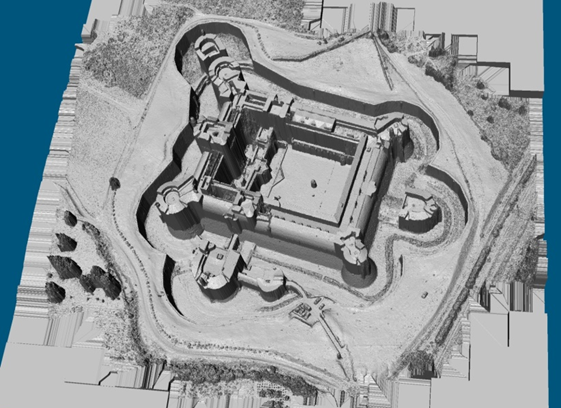
\includegraphics[width=\columnwidth]{example-image-1}
		\end{column}
		\begin{column}{0.33\textwidth}
			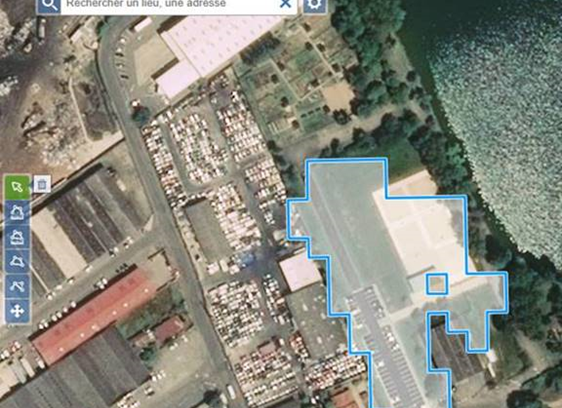
\includegraphics[width=\columnwidth]{example-image-2}
		\end{column}
		\begin{column}{0.33\textwidth}
			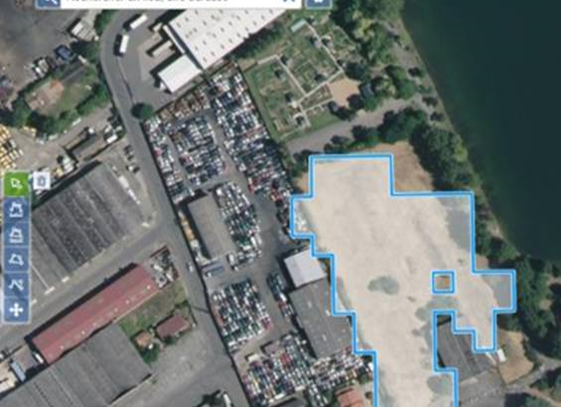
\includegraphics[width=\columnwidth]{example-image-3}
		\end{column}
	\end{columns}

\end{frame}
%%%%%%%%%%%%%%%%%%%%%%%%%%%%%%%%%%%
\begin{frame}

	\frametitle{Tables}
	\framesubtitle{Don't use vanilla \LaTeX{}  tables please}
	
		\begin{center}
			\begin{tabular}{@{}llr@{}}
				\toprule\multicolumn{2}{c}{Item} \\
				\cmidrule(r){1-2}Animal & Description & Price (\$)\\
				\midrule
				Gnat  & per gram  & 13.65 \\
				& each      & 0.01 \\
				Gnu   & stuffed   & 92.50 \\
				Emu   & stuffed   & 33.33 \\
				Armadillo & frozen & 8.99 \\
				\bottomrule
			\end{tabular}
		\end{center}

\end{frame}

\section{URLs and links}
%%%%%%%%%%%%%%%%%%%%%%%%%%%%%%%%%%%
\begin{frame}{Clickable links}

	Lorem ipsum dolor sit amet, consectetur adipiscing elit, sed do eiusmod tempor incididunt ut labore et dolore magna aliqua. 
	Ut enim ad minim veniam, quis nostrud exercitation...
	
	\medskip

	\url{http://www.umr-lastig.fr/seminars}
	
	\href{http://www.umr-lastig.fr/seminars}{Our Thematic Seminars !}
	
	\email{dir-lastig@ign.fr}

\end{frame}

\begin{closingframe}

\Large{\textcolor{LASTIGBlue}{\insertshorttitle}}\\
\bigskip
\large{\textcolor{LASTIGRed}{Thank you for your attention !}}\\
\bigskip
\normalsize
\textbf{Ana-Maria Raimond}\\
Univ Gustave Eiffel, IGN, ENSG, LASTIG\\
\email{dir-lastig@ign.fr}\\
\url{http://www.umr-lastig.fr}

\end{closingframe}


\begin{closingframe}

	You can edit the content of the \texttt{closingframe} environment to design your own closing frame. Example:
	
	\vspace{15mm}

	\begin{columns}
		\begin{column}{0.55\textwidth}
			\raggedleft
			
\includegraphics[width=45mm]{LASTIG_latex_template/elements/logo_uge} 
		\end{column}
		\begin{column}{0.4\textwidth}
			\textbf{Author name}\\
			\email{firstname.lastname@ensg.eu}	
		\end{column}
	\end{columns}

	\vspace{20mm}
			
\end{closingframe}


\end{document}